\newpage

\section{SSA-Style optimizations}

\subsection{Constant Propagation}
\begin{note}{notes}
\begin{itemize}
    \item If  v $\gets$ c , replace all uses of v with c 
    \item If  v $\gets$  $\Phi$ (c,c,c)  (each input is the same constant), replace all uses of v with c
\end{itemize}
\end{note}


\begin{algorithm}
\caption{SSA-CP}\label{alg:SSA-CP}
\begin{algorithmic}
\State{W $\gets$ ist of all defs}
\While{!W.isEmpty}

\State{Stmt S $\gets$ W.removeOne}
\If{(S has form v $\gets$ c) or
(S has form v $\gets$ $\Phi$(c,...,c))}
\State delete S
\For{each stmt U that uses v}
\State {replace v with c in U}
\State {W.add(U)}
\EndFor
\EndIf
\EndWhile

\end{algorithmic}
\end{algorithm}

\subsection{Conditional Constant Propagation }

Wegman and Zadeck's Sparse Conditional Constant (SCC) algorithm was used to find constant expressions, constant conditions, and unreachable code [WZ91]. The output of the SCC algorithm is an association of variables to one of $\lbrace \bot, c, \top \rbrace$, where $\bot$ marks a variable that can hold different values at different times, and $\top$ means the variable is not executed. In addition, every flow-graph node (corresponding to a quadruple) is marked as executable or non-executable. We then walk the flow-graph, eliminating dead-code (quadruples marked non-executable), replacing constant variables with their values, and changing constant conditional branches to goto statements.

\begin{note}{notes}
\begin{itemize}
    \item Assume all blocks unexecuted until proven otherwise
    \item Assume all variables are not executed (only with proof of assignment of a non-constant value do we assume not constant)
\end{itemize}
\end{note}

\subsubsection{Example}

\begin{figure}[H]
    \centering
     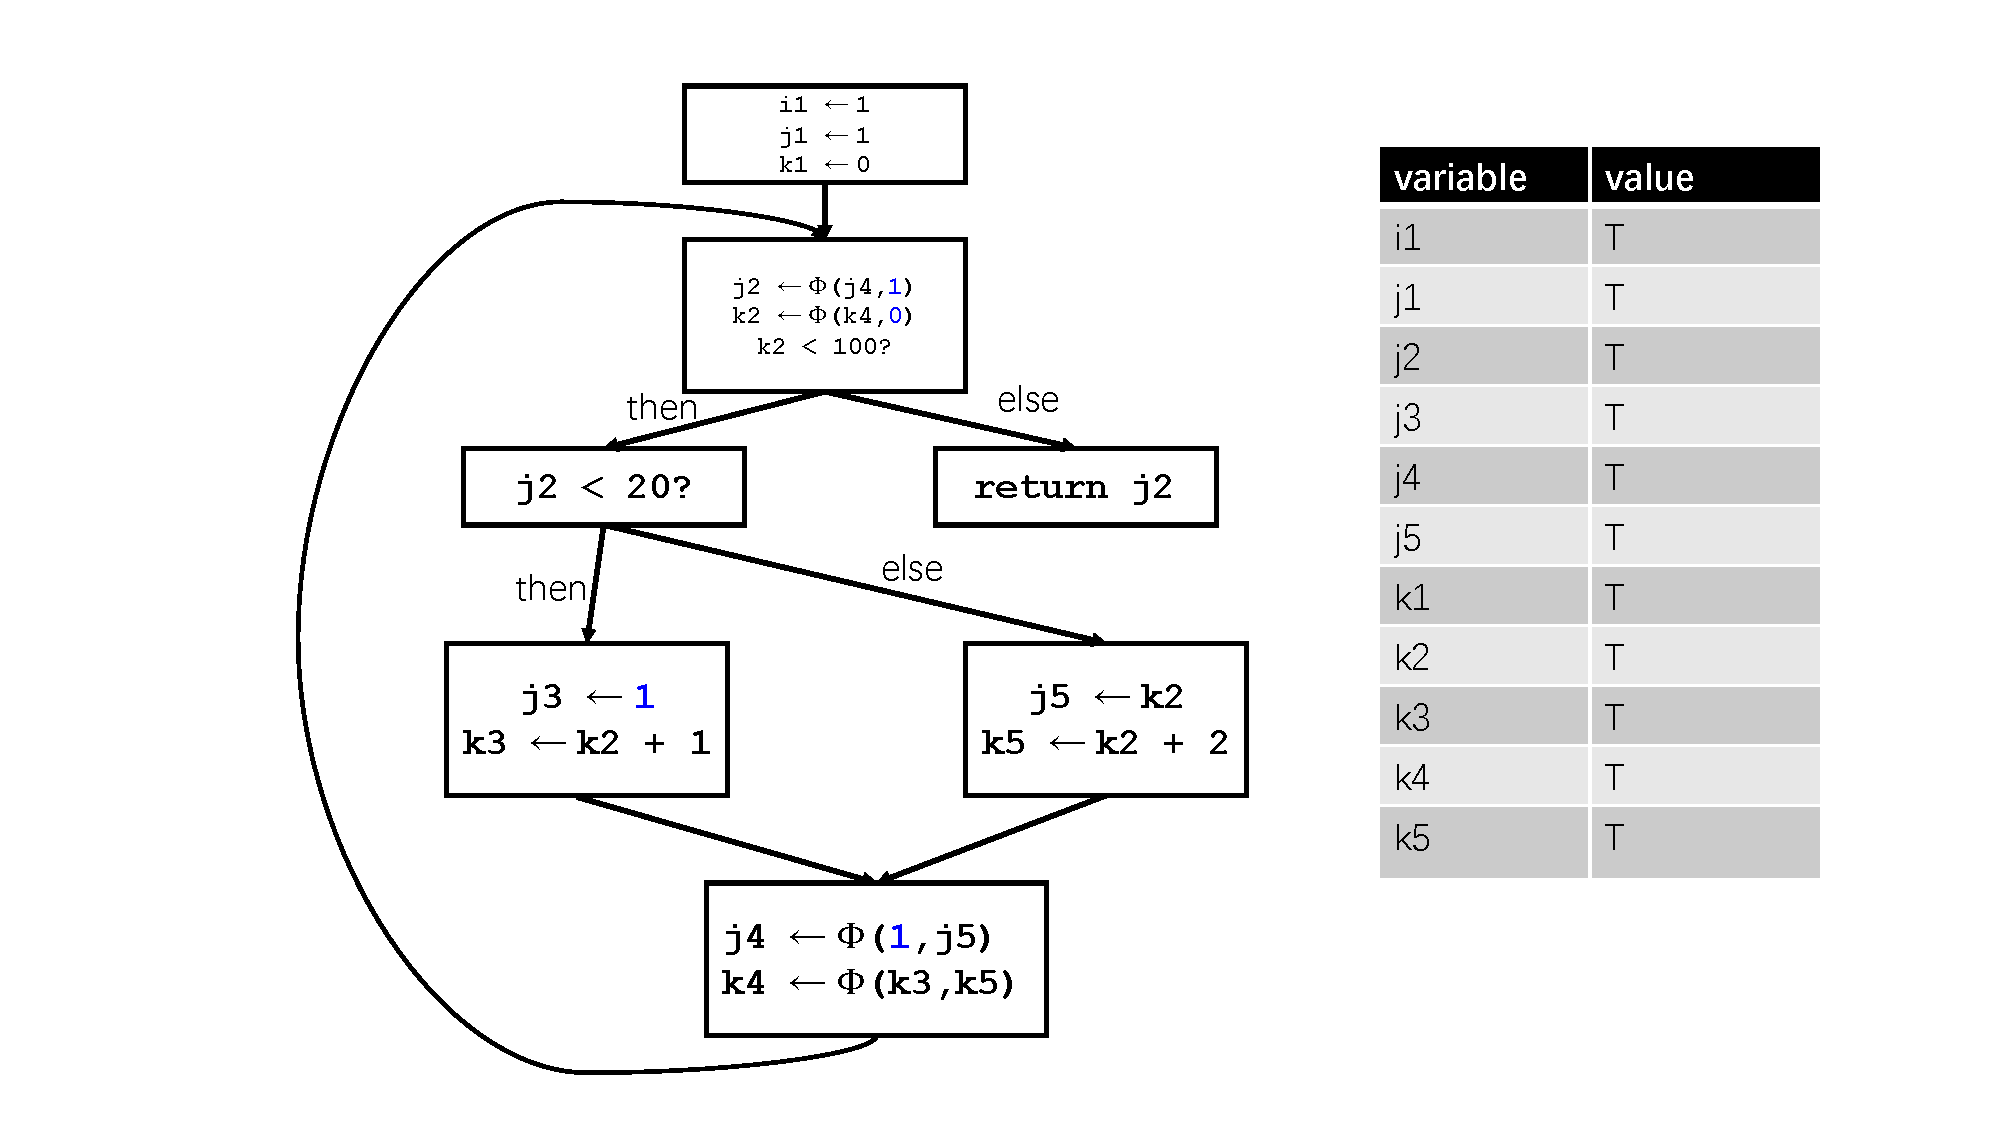
\includegraphics[width=\textwidth]{p47.pdf}
         \caption{Original code. The black block is marked as unexecuted}
         \label{fig:p47}

\end{figure}




\begin{figure}[H]
    \centering
     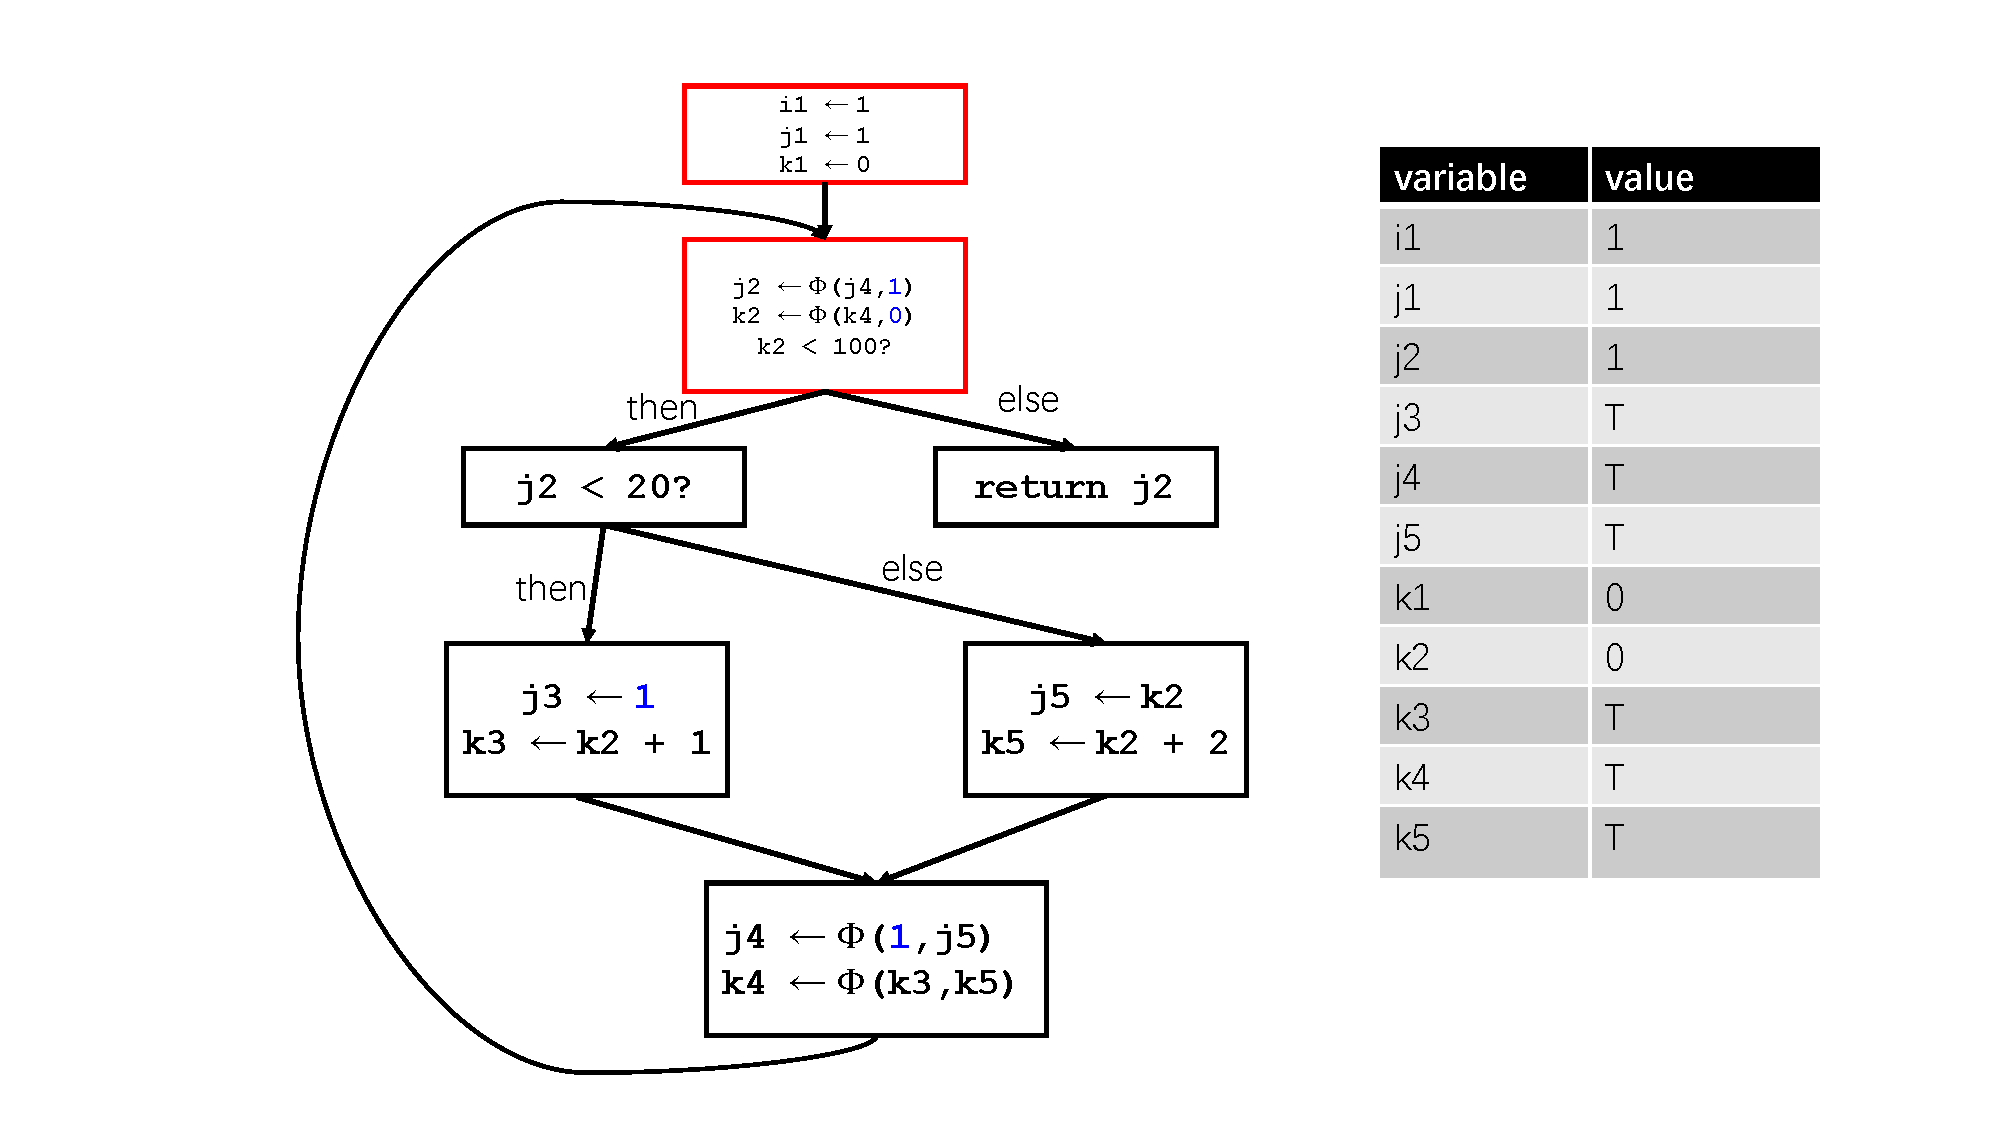
\includegraphics[width=0.8\textwidth]{p48.pdf}
         \caption{The read block is marked as executed. After walking the first two blocks, the value is shown above.}
         \label{fig:p48}

\end{figure}



\begin{figure}[H]
    \centering
     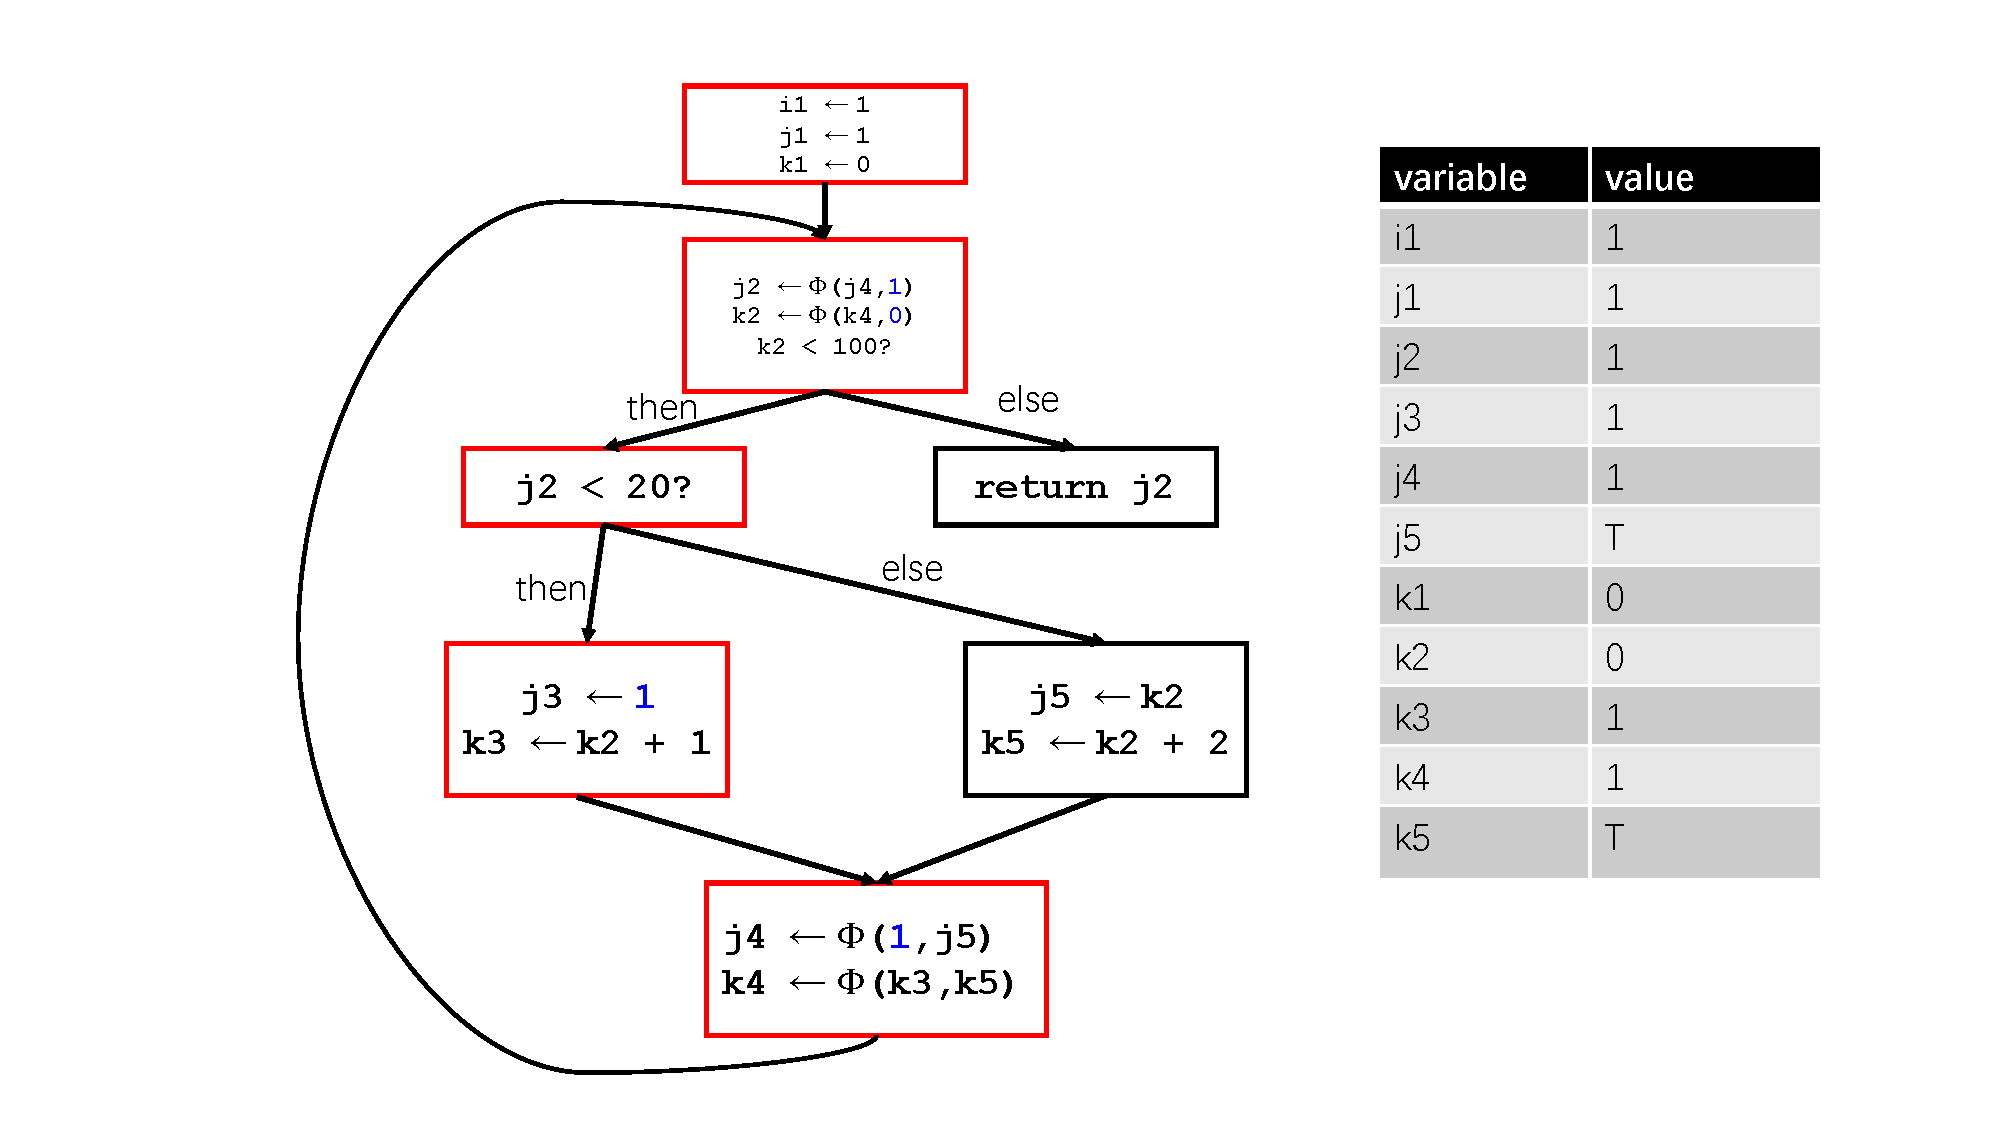
\includegraphics[width=0.8\textwidth]{p49.pdf}
         \caption{After walking 5 blocks.}
         \label{fig:p49}

\end{figure}



\begin{figure}[H]
    \centering
     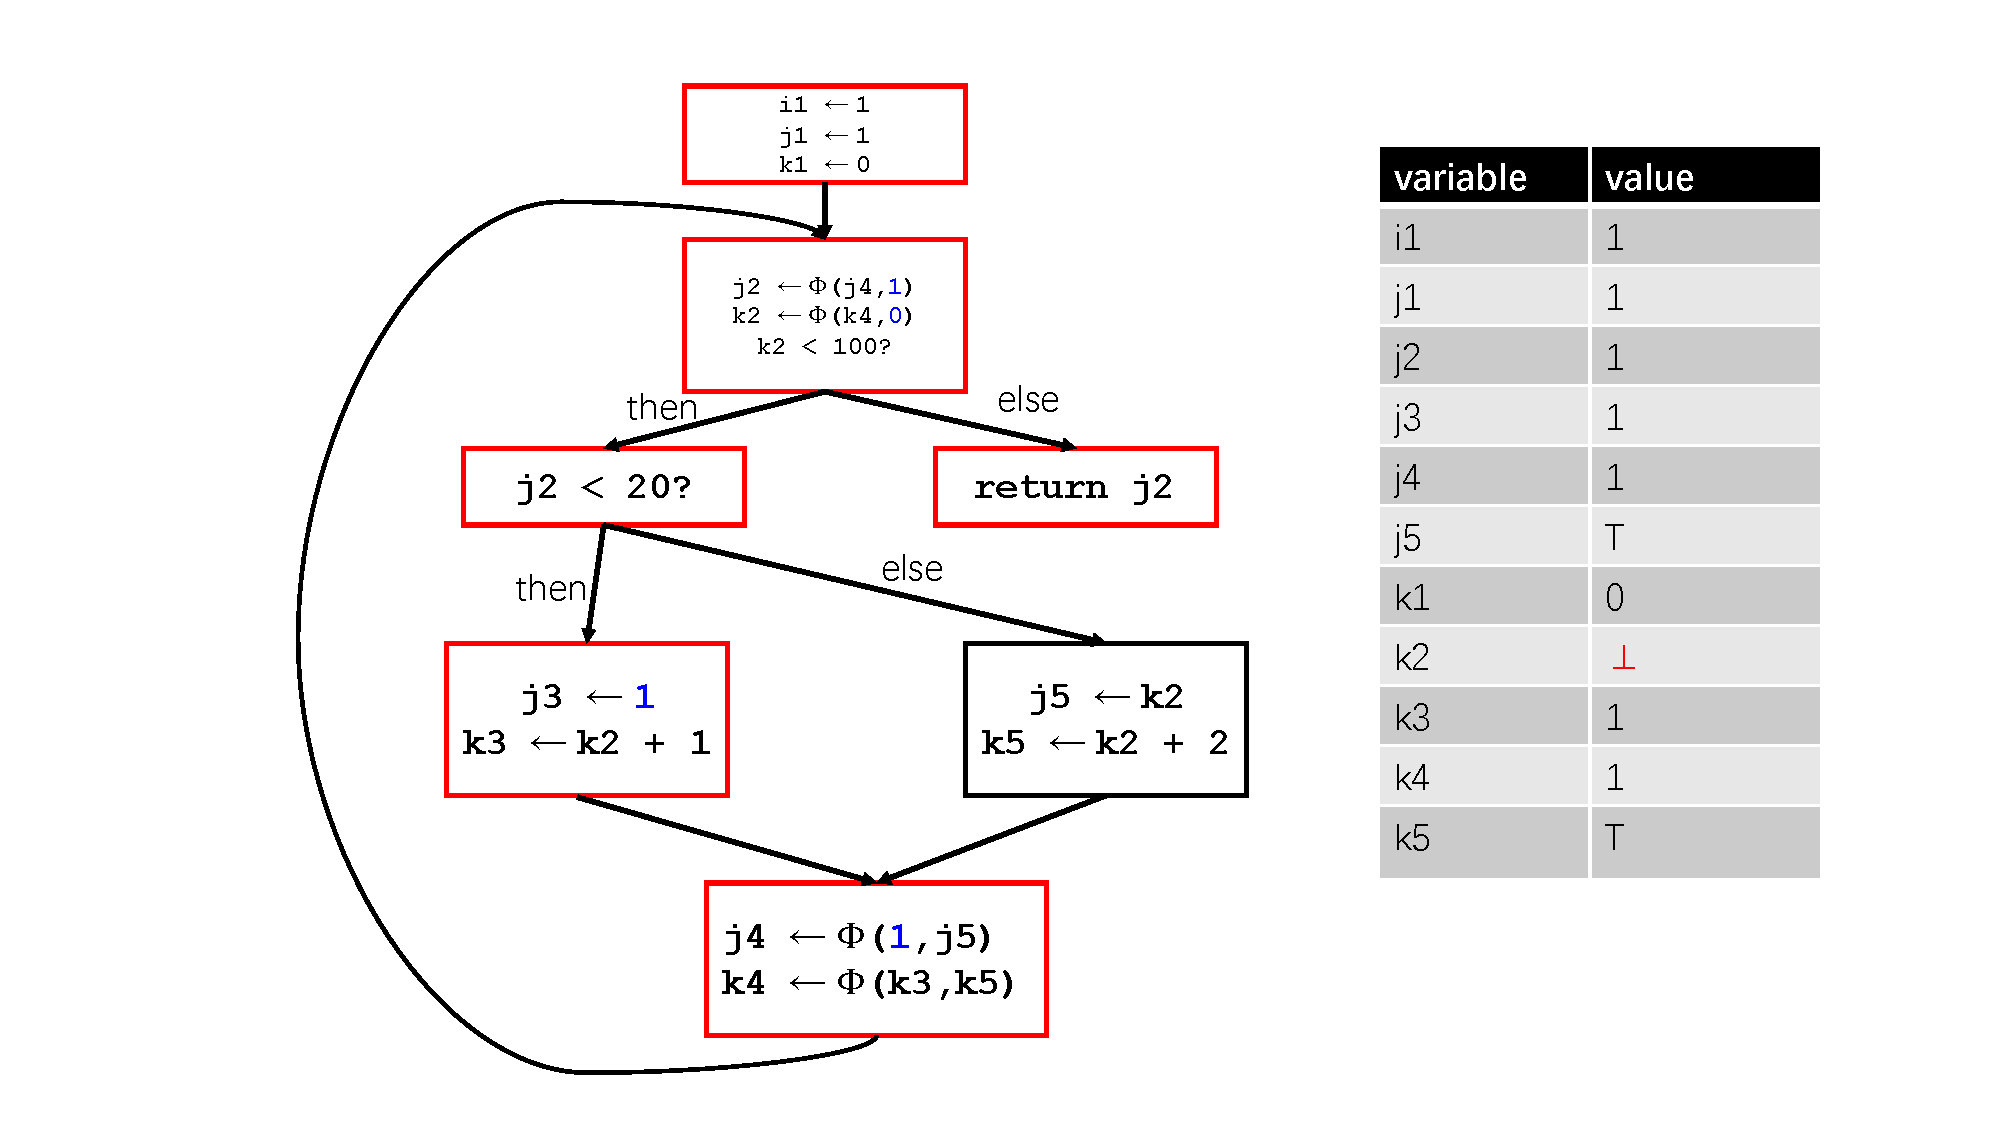
\includegraphics[width=0.8\textwidth]{p50.pdf}
         \caption{Now k2 is $\bot$, so the \texttt{return j2} is reachable.}
         \label{fig:p50}

\end{figure}



\begin{figure}[H]
    \centering
     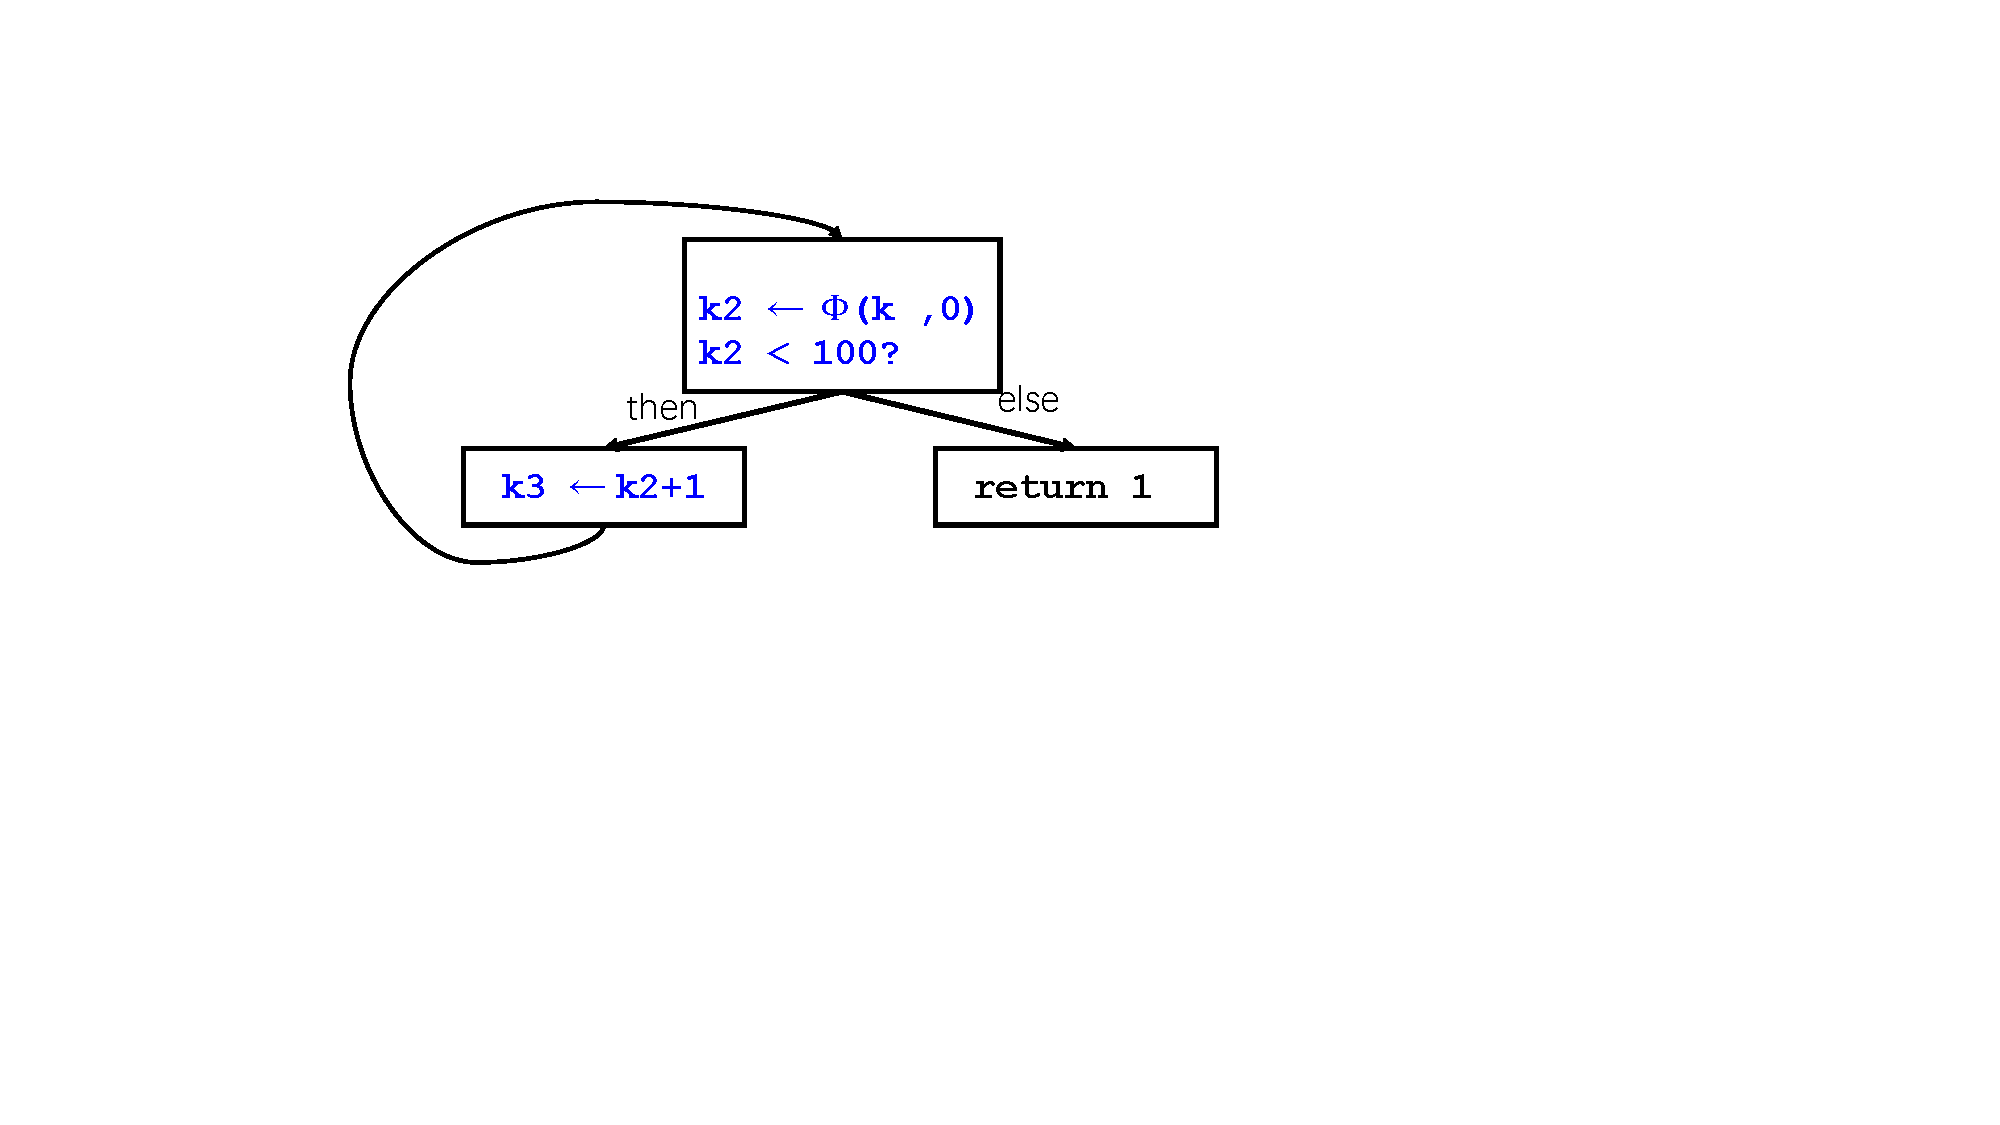
\includegraphics[width=0.5\textwidth]{p51.pdf}
         \caption{Code after applied SCC.}
         \label{fig:p51}

\end{figure}


% \begin{figure}[!b]
%      \centering
%      \begin{subfigure}{0.45\textwidth}
%      \centering
%          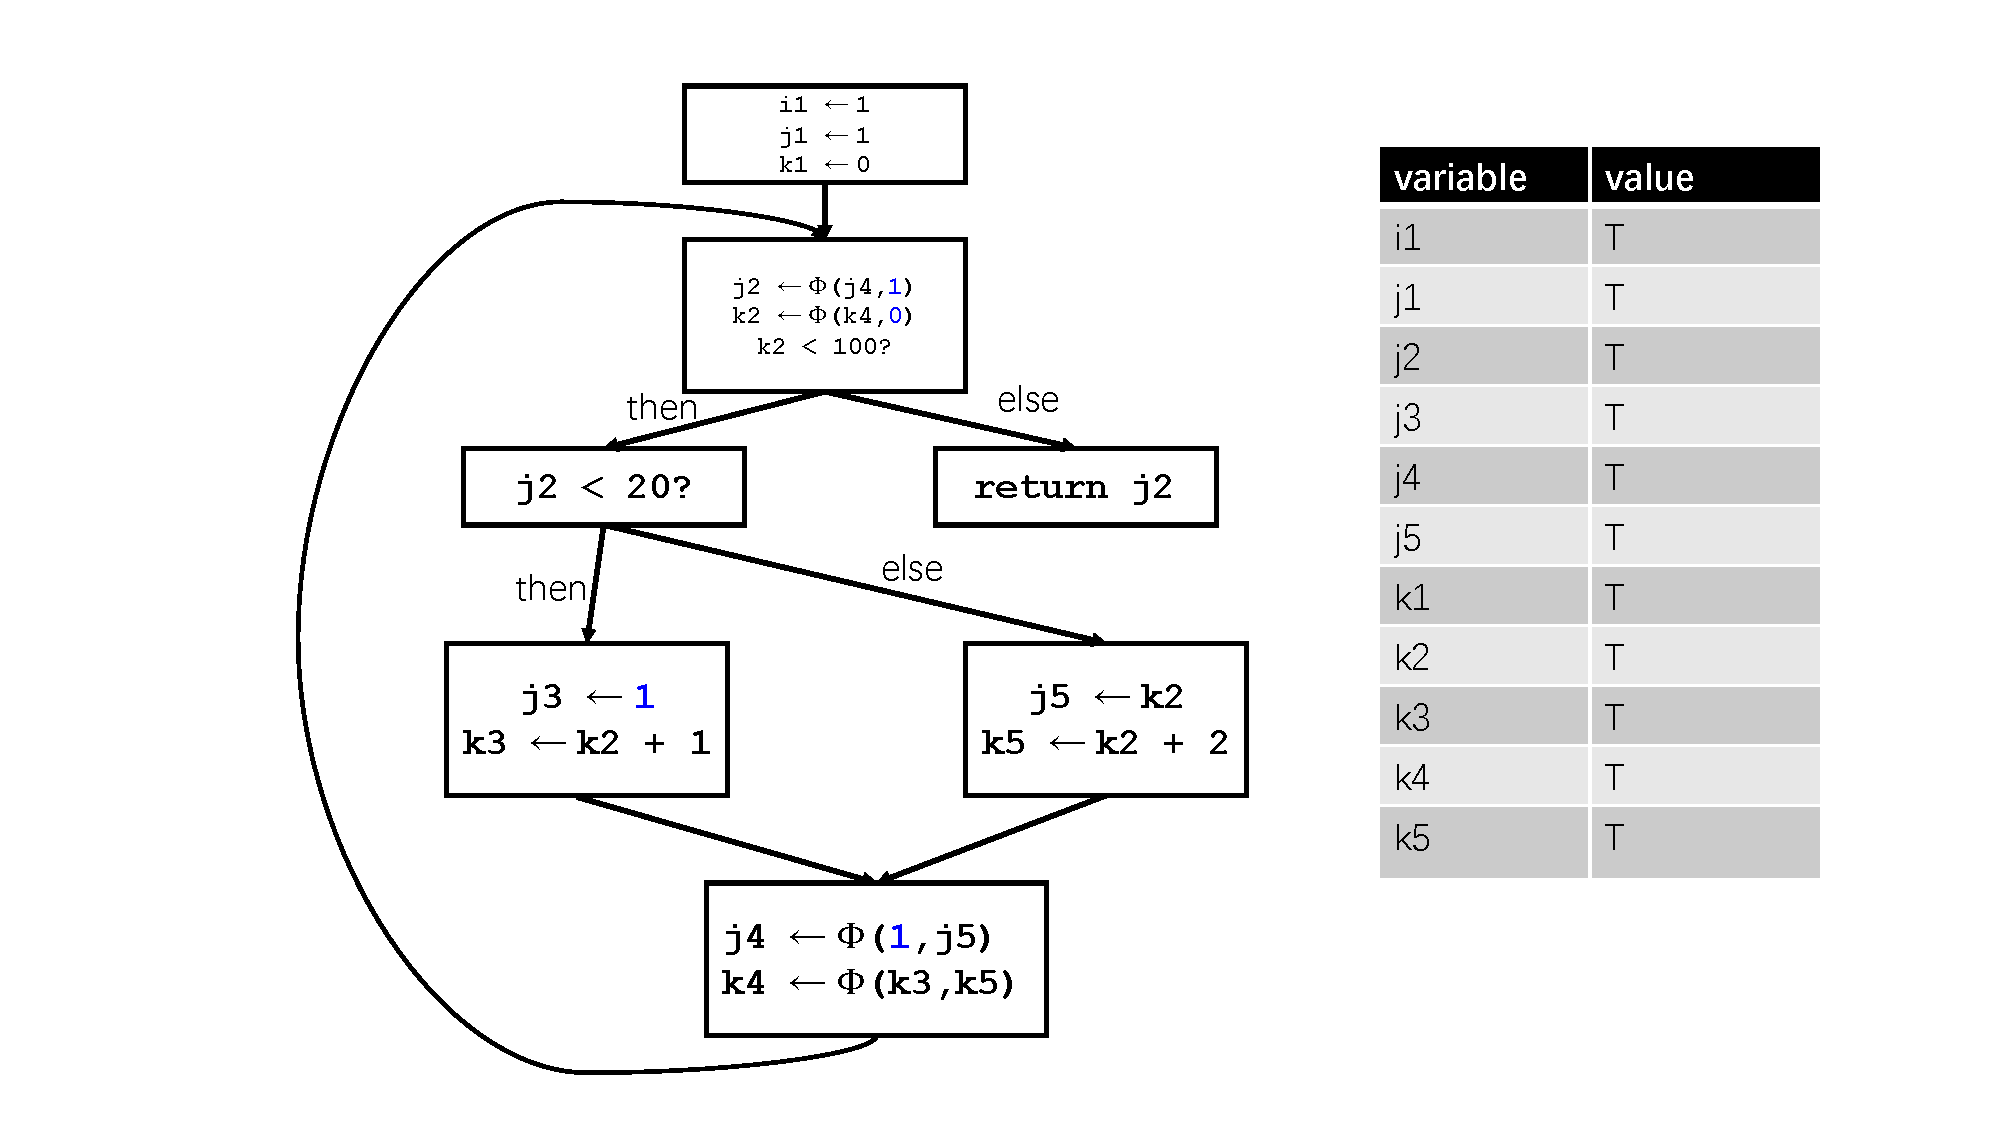
\includegraphics[width=\textwidth]{p47.pdf}
%          \caption{Original code}
%          \label{fig:p47}
%      \end{subfigure}
%      \begin{subfigure}{0.6\textwidth}
%      \centering
%          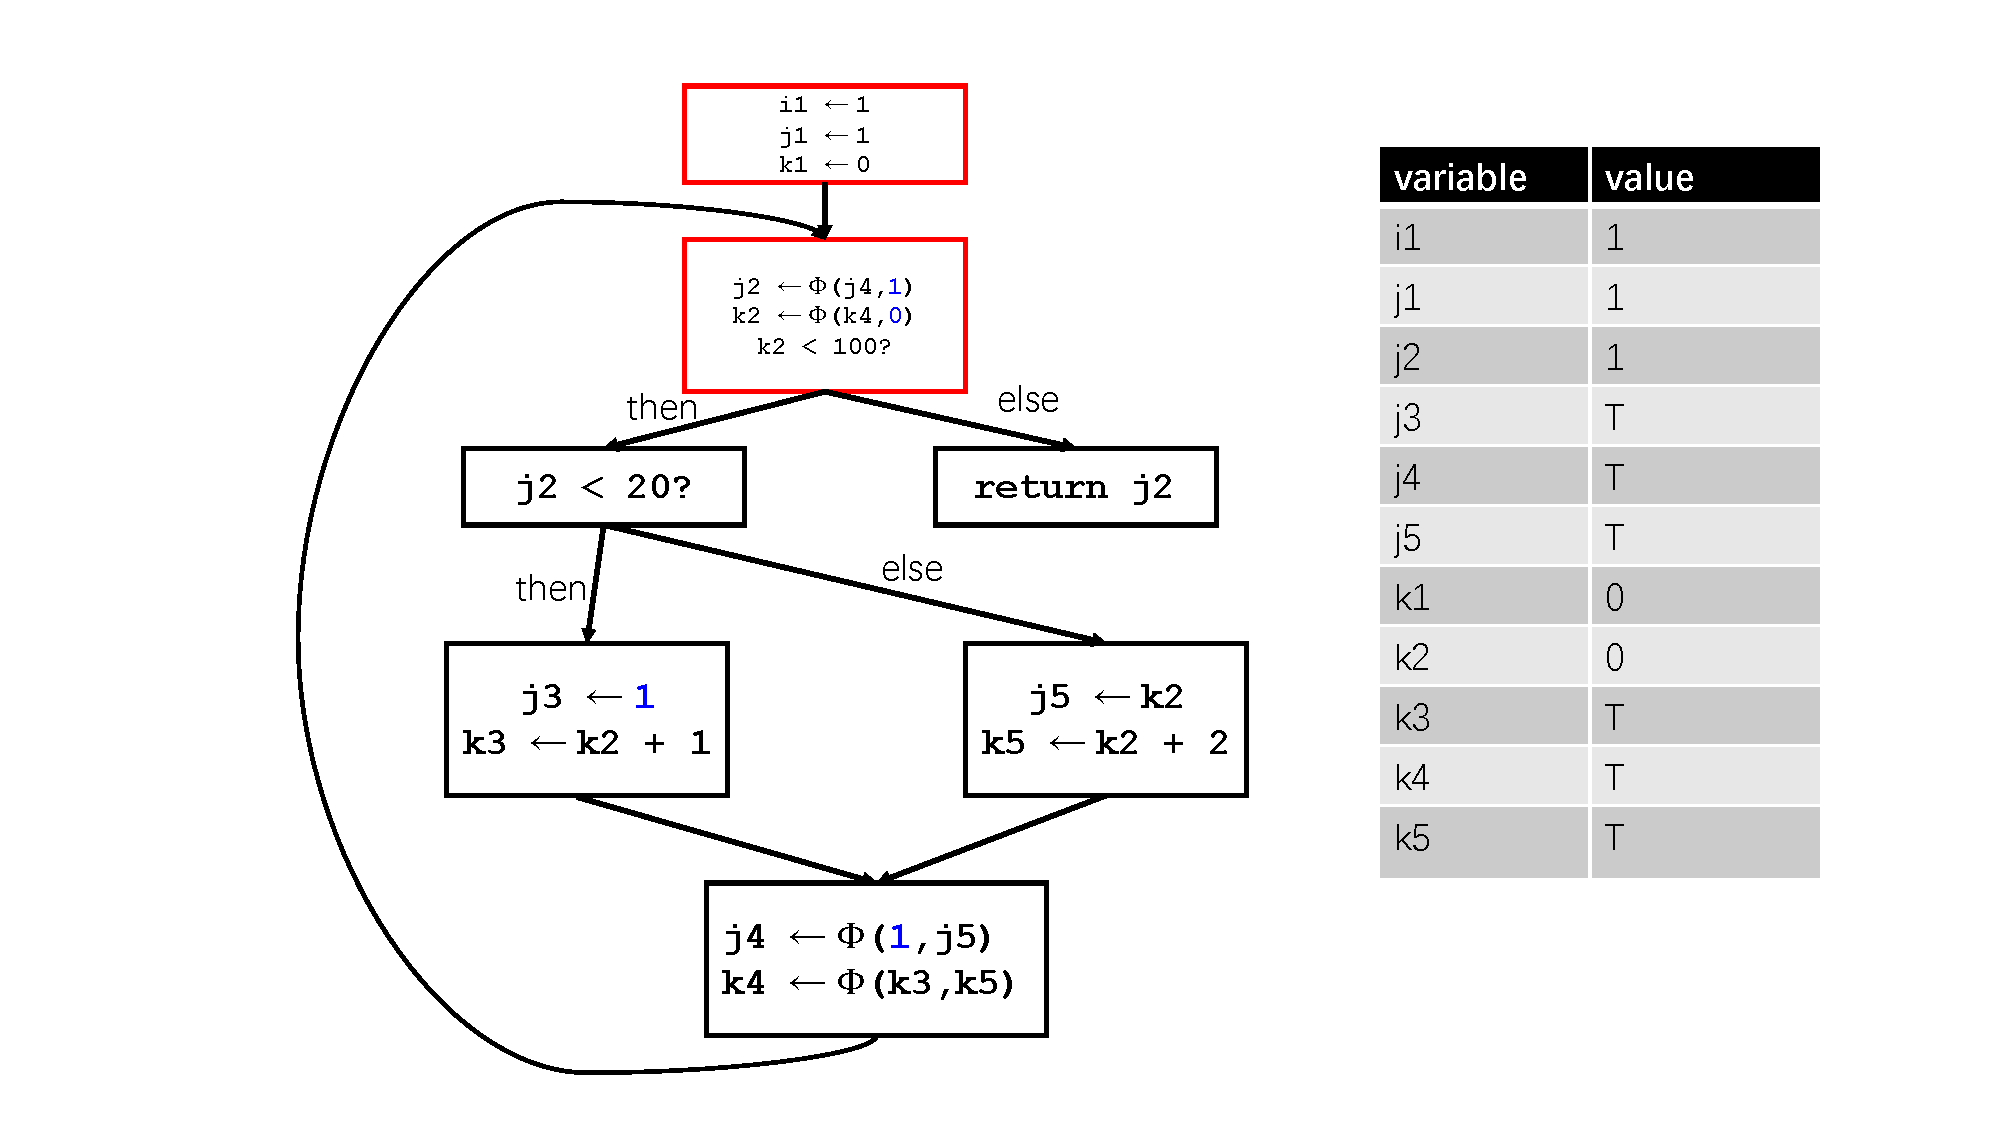
\includegraphics[width=\textwidth]{p48.pdf}
%          \caption{Code after moving instruction.}
%          \label{fig:p48}
%      \end{subfigure}
%           \begin{subfigure}{0.6\textwidth}
%      \centering
%          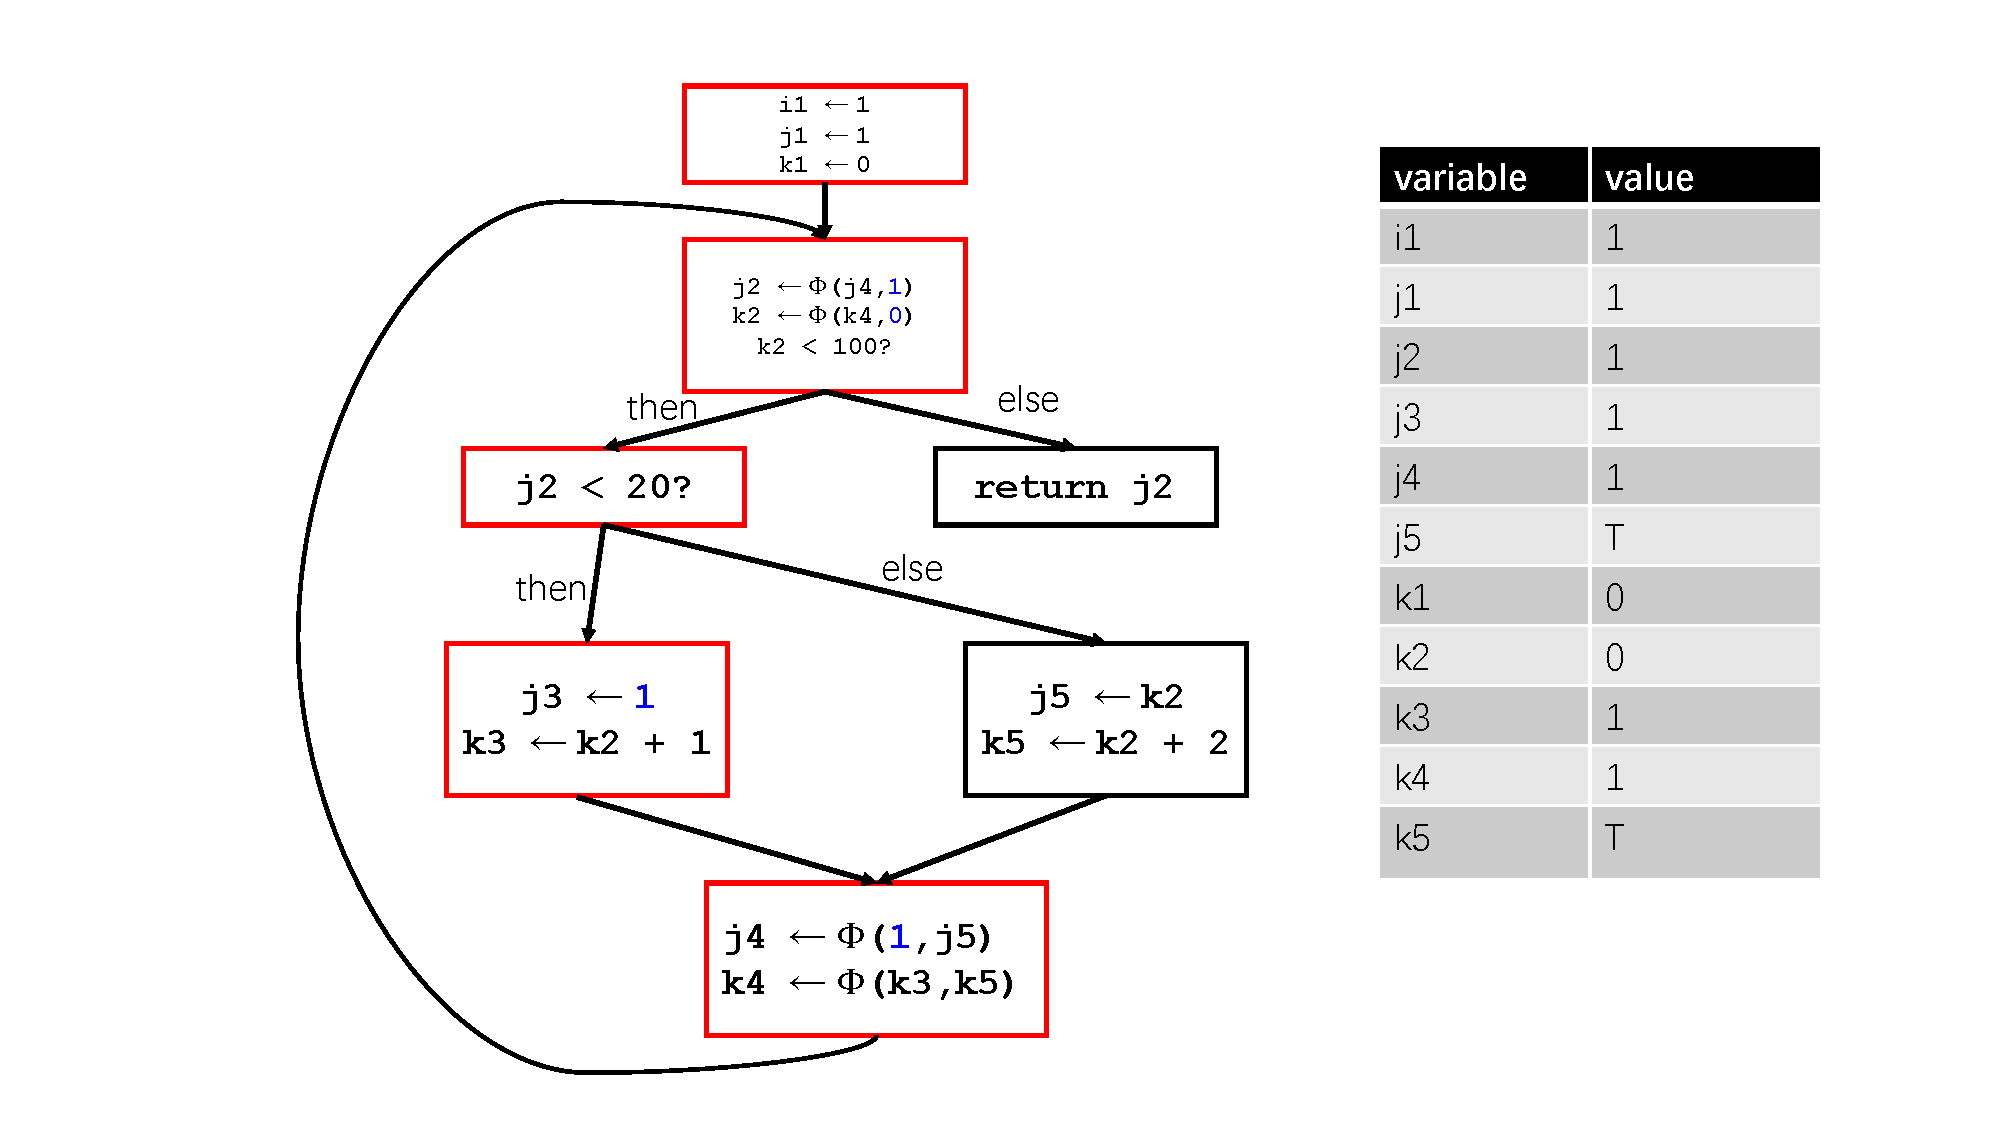
\includegraphics[width=\textwidth]{p49.pdf}
%          \caption{Code after moving instruction.}
%          \label{fig:p49}
%      \end{subfigure}
%           \begin{subfigure}{0.6\textwidth}
%      \centering
%          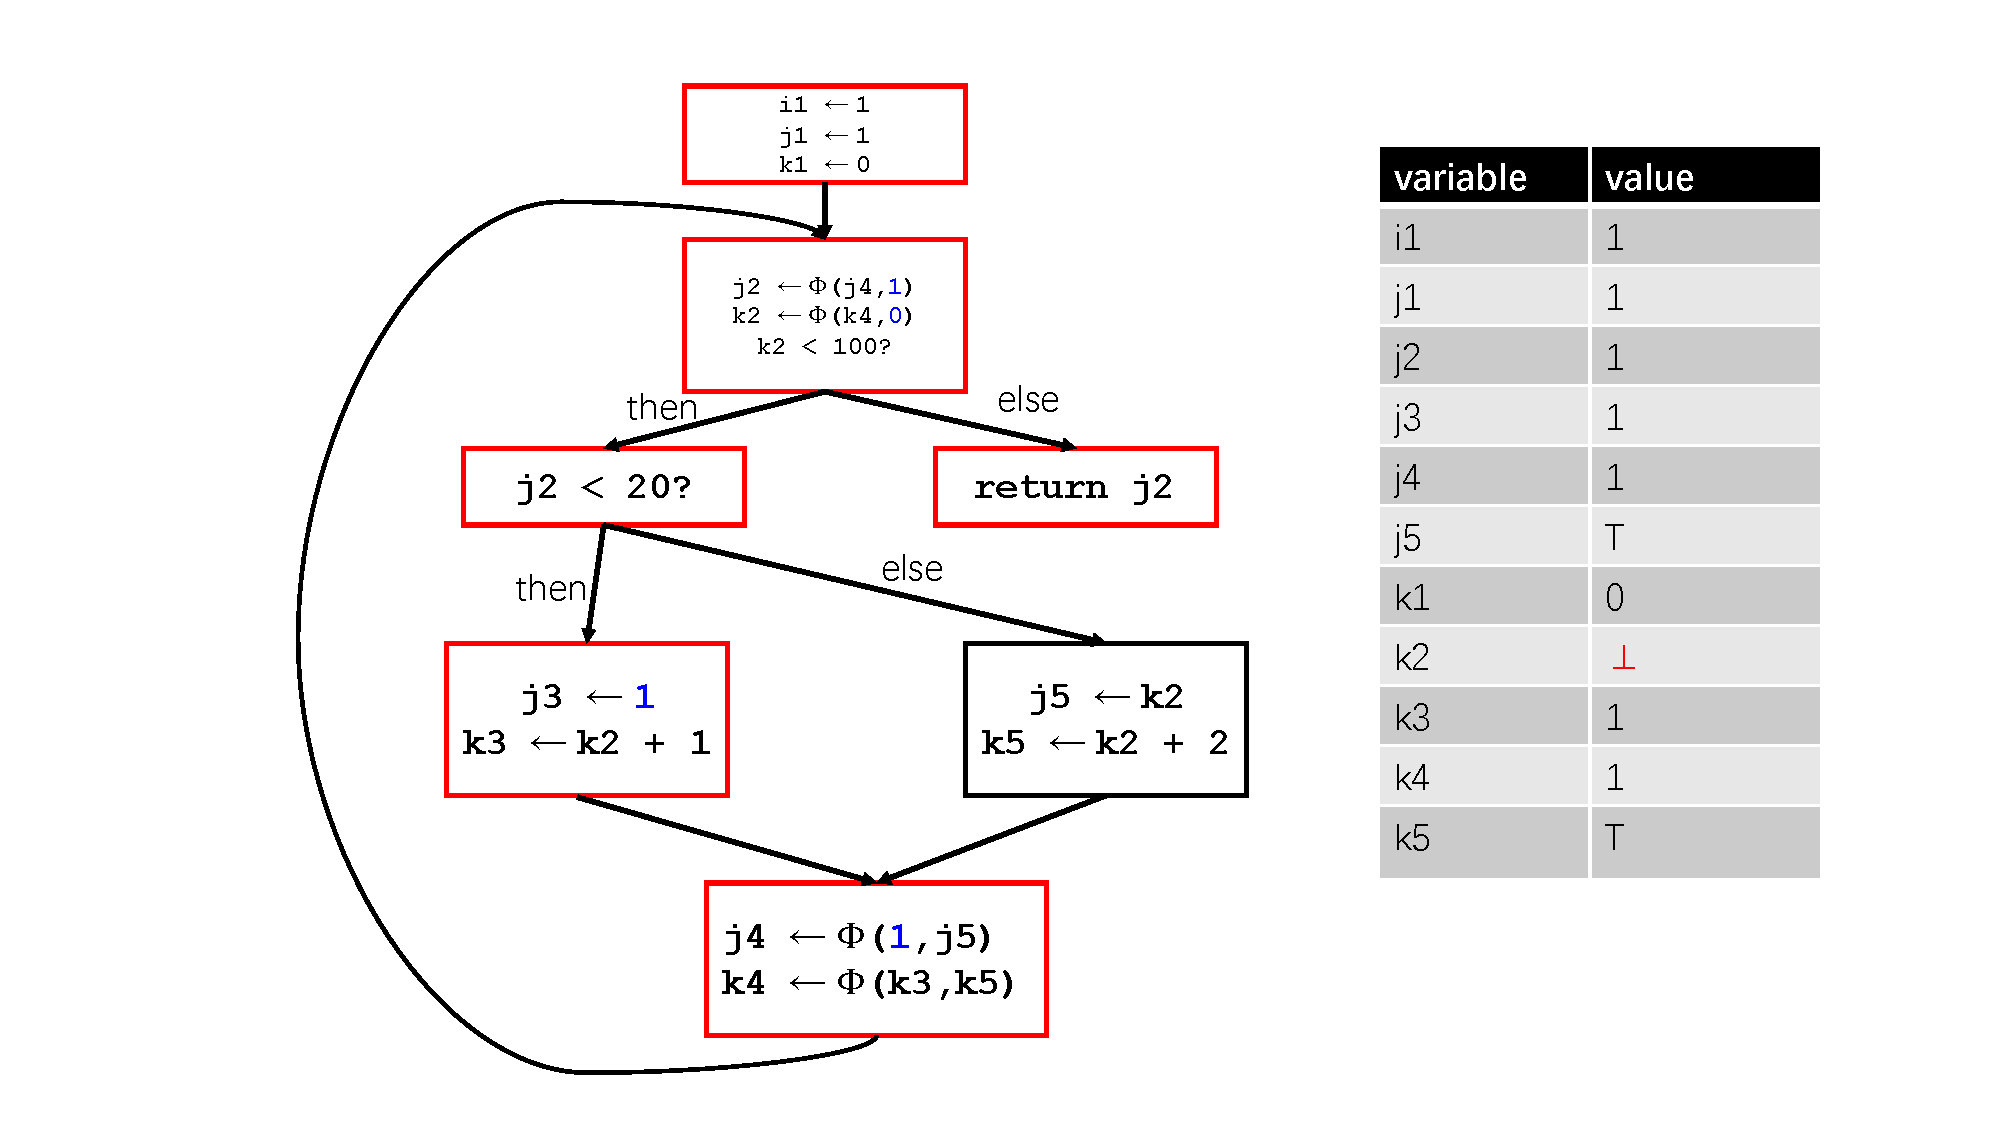
\includegraphics[width=\textwidth]{p50.pdf}
%          \caption{Code after moving instruction.}
%          \label{fig:p50}
%      \end{subfigure}
%           \begin{subfigure}{0.6\textwidth}
%      \centering
%          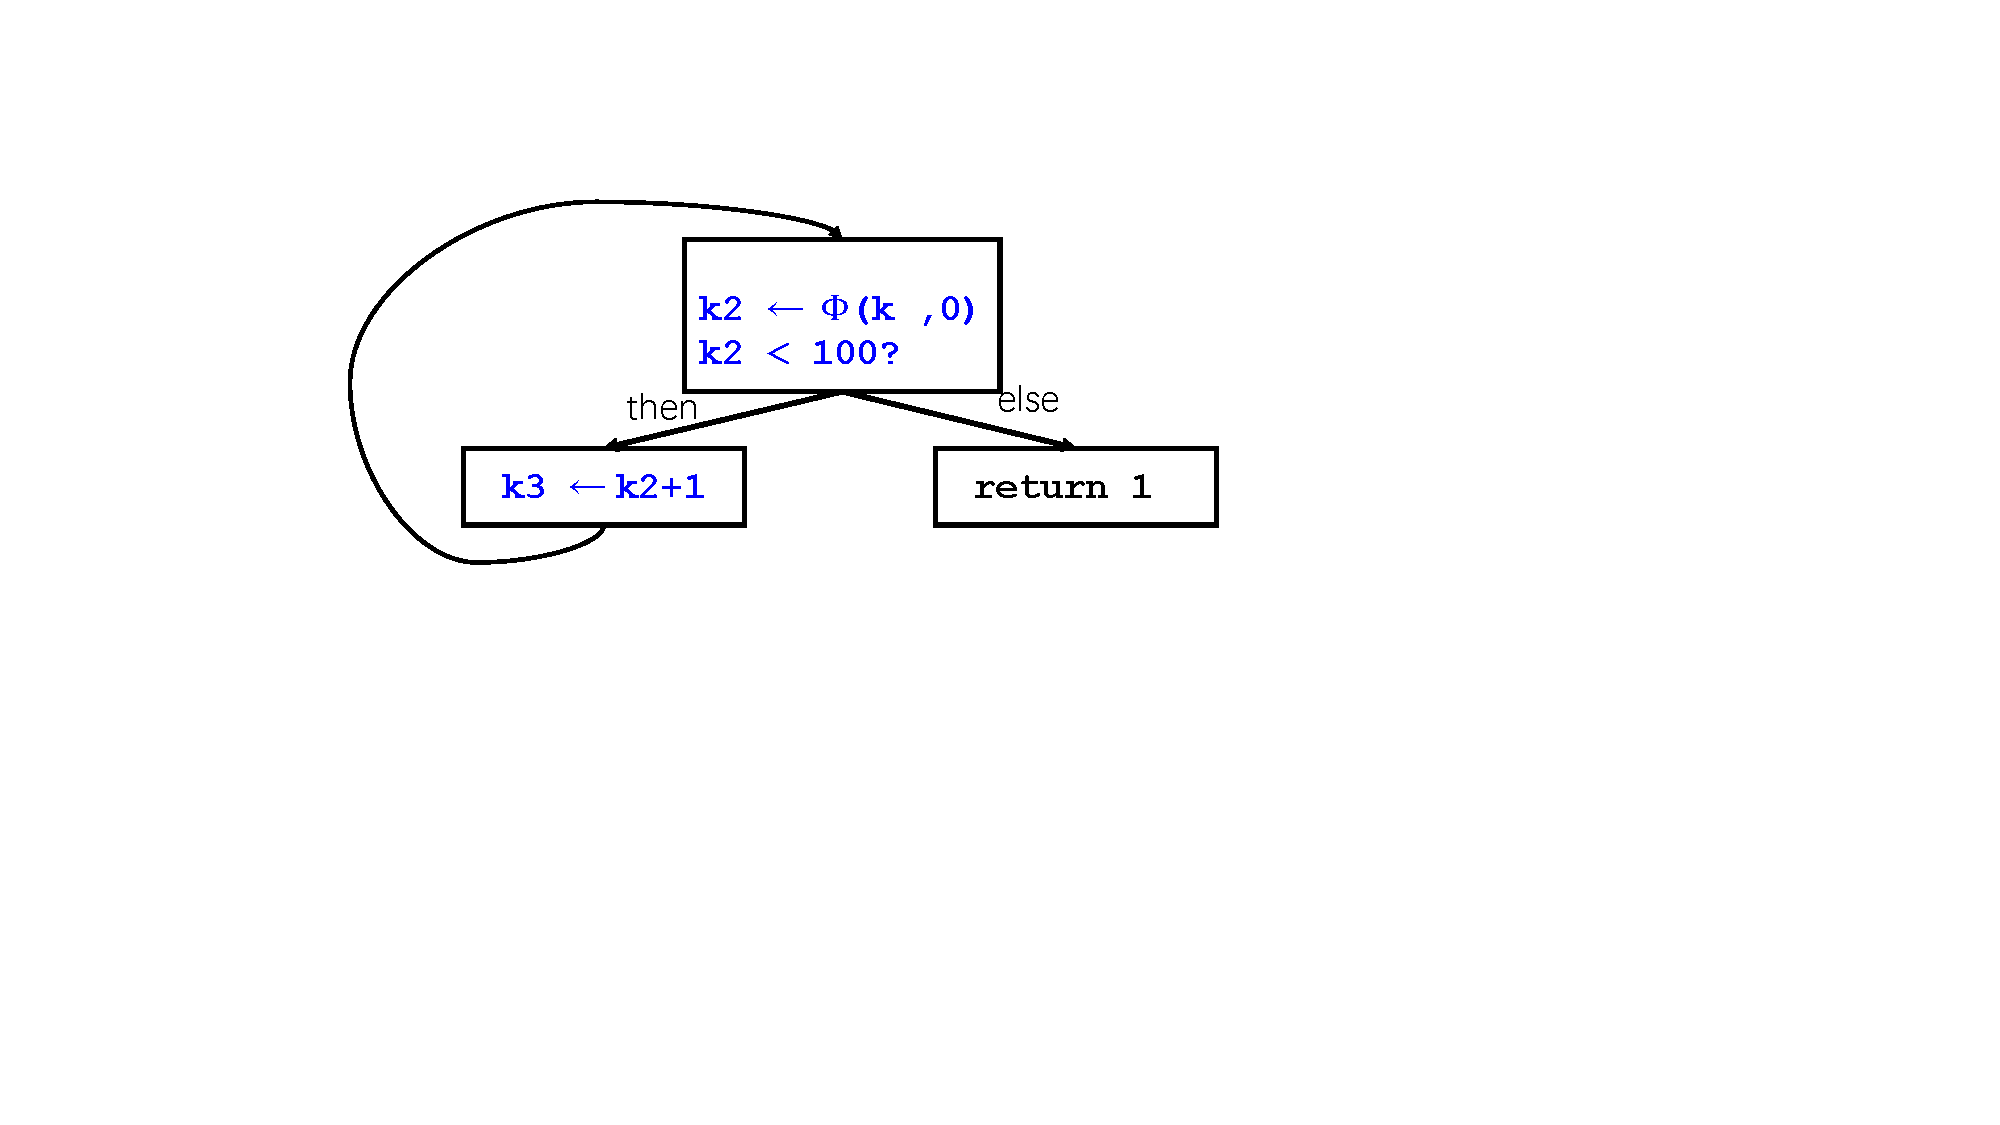
\includegraphics[width=\textwidth]{p51.pdf}
%          \caption{Code after moving instruction.}
%          \label{fig:p51}
%      \end{subfigure}
%         \caption{Implementing $\Phi$-function}
%         \label{fig:p47-51}
% \end{figure}




\subsection{Copy Propogation}

\begin{note}{notes}
\begin{itemize}
    \item  delete x $\gets \Phi$ (y,y,y) and replace all x with y
    \item delete x $\gets$ y and replace all x with y
\end{itemize}
\end{note}






